\documentclass[letterpaper,12pt,twoside=false,DIV=11]{scrbook}

%----------------------CONFIG---------------------------
%math packages
\usepackage{amsmath,amssymb,amsthm,units,unitsdef}

%bibliography style and citation style, bibstyles to use: plainnat, abbrvnat, unsrtnat, named, chicago
%otherwise numerical citationstyle will be used
\usepackage[authoryear,round]{natbib}

\usepackage{longtable,tabularx,tabulary,multirow,lscape}
\usepackage[font={sl},format=plain,labelfont=bf]{caption}

% colors
\usepackage{color,colortbl}
\usepackage[dvipsnames]{xcolor}
\definecolor{darkblue}{HTML}{00354C}

\usepackage{booktabs}
% \usepackage{showkeys} % shows the labels above the references for

%easier development
\usepackage{ifpdf}

\ifpdf
	\usepackage[pdftex]{graphicx}
	\usepackage[]{pdfpages} %for including full pdf pages
	\usepackage[pdftex,
		bookmarks,
		bookmarksopen=true,
		bookmarksnumbered=true,
		pdfauthor={Reto Trappitsch},
		pdftitle={On the origin of elements in the Milky Way},
		colorlinks,
		linkcolor=darkblue,
		citecolor=darkblue,
		filecolor=black,
		urlcolor=darkblue,
		anchorcolor=black,
		menucolor=black,
		breaklinks=true,
		pageanchor=true, %for jumping to a page
		plainpages=false,
		pdfpagelabels=true]{hyperref}
	\pdfcompresslevel=9
	\pdfoutput=1
	\DeclareGraphicsExtensions{.pdf,.png,.jpg,.jpeg}
\else
	\usepackage{graphicx}
\fi
\usepackage{rotating} % rotate figures
\usepackage{subcaption}
\usepackage{wrapfig}

%page style
%==========
%\usepackage{geometry}
%\geometry{top=1.0in, bottom=1.0in, left=1.0in, right=1.0in,footskip = 0.5in} 

% Alert boxes
\usepackage{awesomebox}

% Acronyms
\usepackage{acro}
\acsetup{
	make-links = true
}
% THIS FILE CANNOT BE COMPILED ALONE.

% Declare acronyms below in alphabetical order to use with \usepackage{acro}. 

% DECLARE ACRONYMS %

% NUMBERS
\DeclareAcronym{1d}{short = 2D, long = 1 dimensional}
\DeclareAcronym{2d}{short = 2D, long = 2 dimensional}
\DeclareAcronym{3d}{short = 3D, long = 3 dimensional}

% A
\DeclareAcronym{au}{short = AU, long = astronomical unit, short-plural-form=AU}

% B
\DeclareAcronym{bbn}{short = BBN, long = Big Bang nucleosynthesis}

% C
\DeclareAcronym{cai}{short = CAI, long = calcium-aluminum-rich inclusion}
\DeclareAcronym{ccsn}{short = CCSN, long = core-collapse supernova, short-plural = e, long-plural = e}
\DeclareAcronym{chili}{short = CHILI, long = Chicago instrument for laser ionization}
\DeclareAcronym{cmb}{short = CMB, long = cosmic microwave background}
\DeclareAcronym{cre}{short = CRE, long = cosmic ray exposure}

% D
\DeclareAcronym{dex}{short = dex, long = decimal exponent}
\DeclareAcronym{doi}{short = doi, long = digital object identifier}

% E
\DeclareAcronym{ecsn}{short = ECSN, long = electron-capture supernova, short-plural = e, long-plural = e}
\DeclareAcronym{euv}{short = EUV, long = extreme ultraviolet}

% F
\DeclareAcronym{fip}{short = FIP, long = first ionization potential}
\DeclareAcronym{fit}{short = FIT, long = first ionization time}

% G
\DeclareAcronym{gce}{short = GCE, long = galactic chemical evolution}
\DeclareAcronym{gcr}{short = GCR, long = galactic cosmic ray}
\DeclareAcronym{gw}{short = GW, long = gravitational wave}

% H
\DeclareAcronym{hst}{short = HST, long = Hubble Space Telescope}

% I
\DeclareAcronym{icpms}{short = ICP-MS, long = inductively coupled plasma mass spectrometry}
\DeclareAcronym{imf}{short = IMF, long = initial mass function}
% \DeclareAcronym{imf}{short = IMF, long = instrumental mass fractionation}
\DeclareAcronym{ir}{short = IR, long = infrared radiation}
\DeclareAcronym{ism}{short = ISM, long = interstellar medium}

% J

% K

% L
\DeclareAcronym{ligo}{short = LIGO, long = laser interferometer gravitational-wave observatory}
\DeclareAcronym{lion}{short = LION, long = laser ionization of neutrals}
\DeclareAcronym{lte}{short = LTE, long = local thermodynamic equilibrium}

% M
\DeclareAcronym{mesa}{short = MESA, long = Modules for Experiments in Stellar Astrophysics}
\DeclareAcronym{mc}{short = MC, long = Monte Carlo}
\DeclareAcronym{mswd}{short = MSWD, long = mean square weighted deviation}

% N
\DeclareAcronym{nanosims}{short = NanoSIMS, long = nanoscale secondary ion mass spectrometry}
\DeclareAcronym{nlte}{short = NLTE, long = nonplocal thermodynamic equilibrium}
\DeclareAcronym{ns}{short = NS, long = neutron star}

% O
\DeclareAcronym{odr}{short = ODR, long = orthogonal distance regression}

% P
\DeclareAcronym{pc}{short = pc, long = parsec}
\DeclareAcronym{pdf}{short = pdf, long = portable document format}
\DeclareAcronym{pdfstat}{short = PDF, long = probability density function}

% Q

% R
\DeclareAcronym{rims}{short = RIMS, long = resonance ionization mass spectrometry}
\DeclareAcronym{rproc}{short = \textit{r}-process, long = rapid neutron capture process, short-plural = es, long-plural = es}
\DeclareAcronym{rsf}{short = RSF, long = relative sensitivity factor}

% S
\DeclareAcronym{scr}{short = SCR, long = solar cosmic ray}
\DeclareAcronym{sep}{short = SEP, long = solar energetic particle}
\DeclareAcronym{slr}{short = SLR, long = short-lived radionuclide}
\DeclareAcronym{sfr}{short = SFR, long = star formation rate}
\DeclareAcronym{sims}{short = SIMS, long = secondary ion mass spectrometry}
\DeclareAcronym{soho}{short = SOHO, long = solar and heliospheric observatory}
\DeclareAcronym{sn}{short = SN, long = supernova, short-plural = e, long-plural = e}
\DeclareAcronym{snia}{short = SN-Ia, long = type Ia supernova, short-plural-form = SNe-Ia, long-plural = e}
\DeclareAcronym{snii}{short = SN-II, long = type II supernova, short-plural-form = SNe-II, long-plural = e}
\DeclareAcronym{sproc}{short = \textit{s}-process, long = slow neutron capture process, short-plural = es, long-plural = es}
\DeclareAcronym{sw}{short = SW, long = solar wind}

% T
\DeclareAcronym{tof}{short = TOF, long = time-of-flight}

% U
\DeclareAcronym{uv}{short = UV, long = ultraviolet}

% V

% W
\DeclareAcronym{wd}{short = WD, long = white dwarf}
\DeclareAcronym{wmap}{short = WMAP, long = Wilkinson microwave anisotropy probe}

% X

% Y

% Z

% newcommands
%============
% my short cuts
\providecommand{\e}[1]{\ensuremath{\times 10^{#1}}}
\providecommand{\ex}[1]{\ensuremath{^{#1}}}
\providecommand{\dex}[1]{\ensuremath{\delta^{#1}}}
\newcommand{\nean}{$^{22}$Ne($\alpha$,n)$^{25}$Mg}

% textnormal
\newcommand{\tn}{\textnormal}
% textregistered
\newcommand{\tr}{$^\tn{\textregistered}$}

% more box stuff
\makeatletter
\providecommand{\boxtitle}[1]{\sffamily{\textbf{#1}}\normalfont}
	
\providecommand{\infobox}[2]{\awesomebox[MidnightBlue]{2pt}{\faPaw}{MidnightBlue}{\boxtitle{#1} #2}}
\providecommand{\morebox}[2]{\awesomebox[BrickRed]{2pt}{\faRocket}{BrickRed}{\boxtitle{#1} #2}}
\providecommand{\codebox}[2]{\awesomebox[OliveGreen]{2pt}{\faCode}{OliveGreen}{\boxtitle{#1} #2}}



%=========================================================================================================
%title specifications

\title{On the Origin of Elements in the Milky Way}
\author{Reto Trappitsch}
\date{Spring semester 2021}




%-------------------DOCUMENT---------------------------

\usepackage{blindtext}
\begin{document}

\maketitle

% TOC
\pagenumbering{roman}
\setcounter{page}{1}
\tableofcontents

\clearpage


% MAIN TEXT
\pagenumbering{arabic}
\setcounter{page}{1}

\chapter*{Preface}\label{sec:preface}
\addcontentsline{toc}{chapter}{Preface}

These lecture notes for the course ``On the origin of the elements in the Milky Way'' are prepared as we go, so they will be in part influenced by you! If you find typos, errors, or other issues please let me know. The most recent copy of the \LaTeX\ files and figures can also be found on \href{https://github.com/galactic-forensics/lecutre_origin_elements/}{GitHub}.

The lecture notes contain clickable links, e.g., all references are linked to the bibliography and all acronyms are linked to the acronyms' definition page. These links are generally colored in \textcolor{darkblue}{dark blue}.

The end of the document contains a bibliography that contains details on all references. Note that references here are limited and often point to review articles that could be of interest to the reader. More detailed references to individual topics can be found in these articles. Each reference entry contains a \acf{doi}\footnote{\url{https://doi.org}} that can be found online and accessed via a Brandeis library subscription. Alternatively, a link to ArXiV\footnote{\url{https://arxiv.org}} is provided.

Specific boxes throughout the text discuss further information. They are defined as following:

\infobox{Background information}{on topics that do not necessarily fit into the text but are important to keep in mind will be given in a box like this.}

\morebox{Further information and reading}{for the avid reader will be pointed out in a box like this. The scope of these boxes is generally slightly outside the realm of the class.}

\codebox{Programming}{is an integral part of scientific research, be it for running experiments, performing measurements, evaluating measurements, or modeling a system. A box like this will point you to more information with respect to coding. These boxes will often refer to coding in \href{https://www.python.org}{python}.}

\printacronyms


% Chapters

%!TEX root = origin_elements_lecture_notes.tex

\chapter{Solar System Abundances}\label{ch:solar_system_abundances}

To understand the origin of the elements in the Milky Way, it is crucial to first understand what in fact needs explaining. One of the best studied points in the history of the Milky Way is the Solar System we inhabit, mainly since we actually live inside it and thus have direct access to its material.

The Solar System formed 4.567\,Ga ago from a homogeneous molecular cloud. Since the Milky Way itself formed roughly 13\,Ga ago, the molecular cloud from which the solar nebula formed evolved for roughly 8.4\,Ga since the formation of the Milky Way and around 9\,Ga since the Big Bang. The process that describes the formation and destruction of elements over this period of time is generally referred to as \ac{gce}. 

\begin{figure}[bt]
    \begin{subfigure}{0.5\textwidth}
        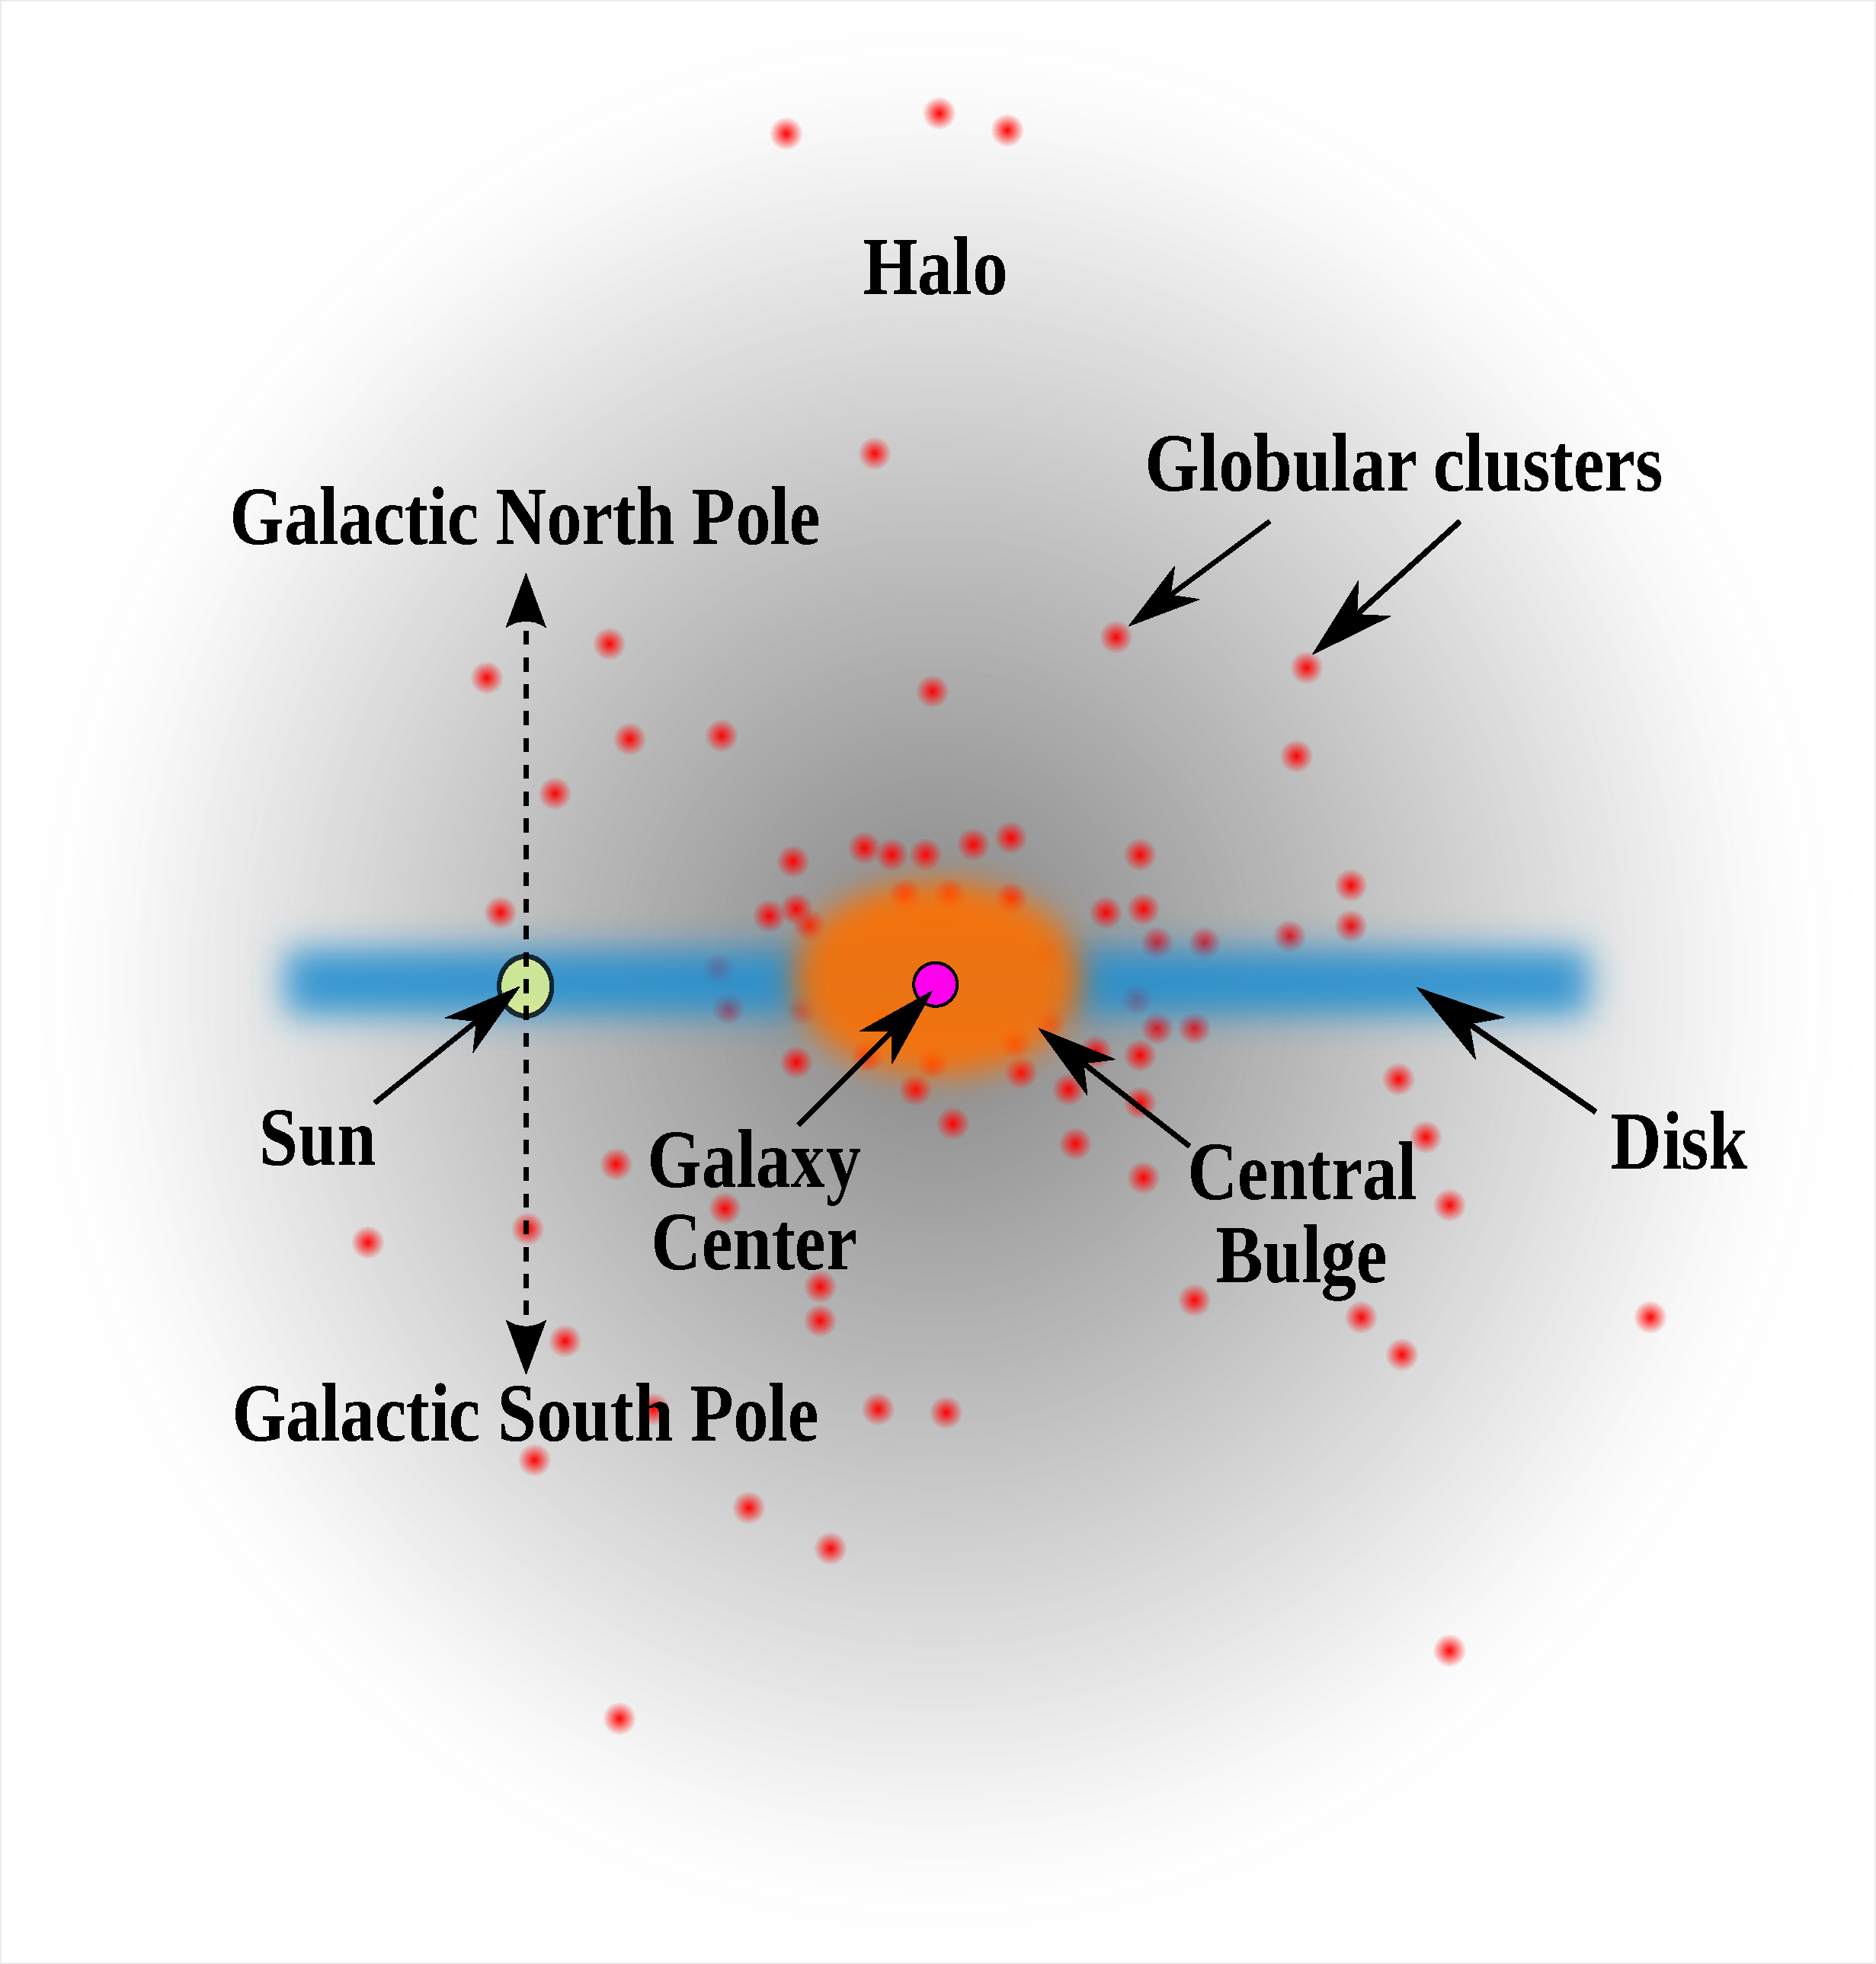
\includegraphics[width=\textwidth]{graphics/solar_system_abundances/milky_way_profile_wiki}
    \end{subfigure}
    \begin{subfigure}{0.5\textwidth}
        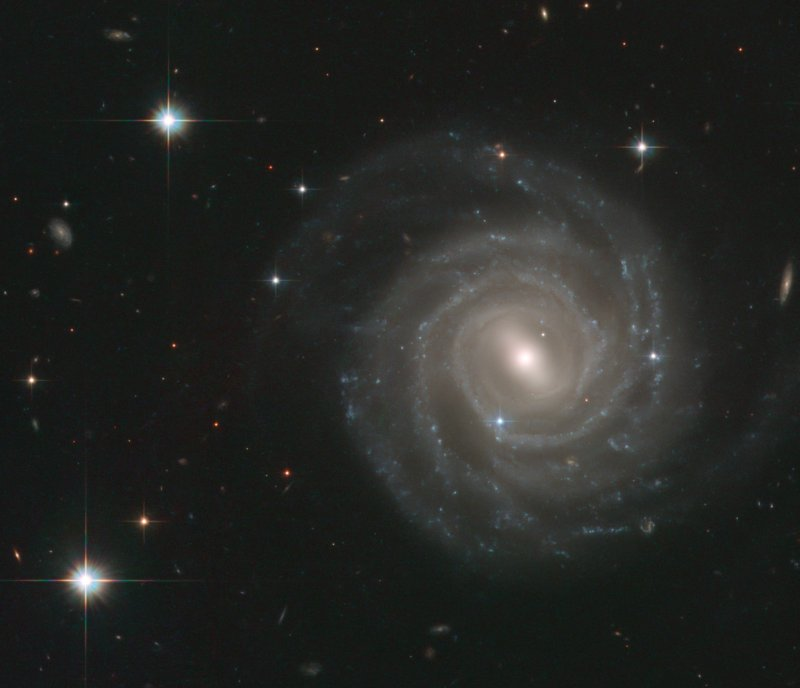
\includegraphics[width=\textwidth]{graphics/solar_system_abundances/UGC_12158}
    \end{subfigure}
    \caption{Left: Profile of the Milky Way with the current position of the Solar System indicated. Edited from \href{https://en.wikipedia.org/wiki/Milky_Way}{Wikipedia}. Right: Galaxy UGC 12158, which is thought to have a similar spiral structure as the Milky Way. Credit: ESA/Hubble \& NASA}
    \label{fig:milky_way_profile_wiki}
\end{figure}
In order to put the Solar System abundances in perspective to the galaxy, Figure~\ref{fig:milky_way_profile_wiki} shows a schematic of the Milky Way (left). The galactic center, which is likely a black hole, is surrounded by an area called the bulge. The disk of the Milky Way has a spiral structure. An analogue galaxy with a similar structure is UGC 12158, shown on the right in Figure~\ref{fig:milky_way_profile_wiki}. The densest regions of the Milky Way are close to the center (e.g., the bulge) while less dense areas are further out (e.g., the disk). The Solar System is located in the disk and about two-thirds out from the center in one of the spiral arms called the Orion-Cygnus arm. Disk and bulge are both surrounded by a low-density halo. This halo also contains globular clusters, which are gravitationally bound aggregations of stars. These clusters tend to be very old and are thus made of material that formed early on in the history of the Milky Way.

This chapter discusses the composition of the Solar System 4.567\,Ga ago (the initial Solar System abundances) and today (abundances in the solar photosphere). While we can observe stars and determine their composition via spectroscopy, the Solar System is unique since we have meteorites available that represent unaltered solar nebula material. This material is especially useful since it can be studied in the laboratory using mass spectrometry techniques. 

\codebox{Initial Solar System abundances in python}{can easily be handled with the \href{https://github.com/galactic-forensics/iniabu}{\texttt{iniabu}} package. This package can be used make various databases of Solar System abundances available for interaction and is used here to create abundance plots using \href{https://www.matplotlib.org}{\texttt{matplotlib}}. Full disclosure: I am the author of the package and am thus surely biased.}


\section{Definitions and Notations}

\subsection{Terminology}

\textbf{Elemental concentrations and abundances} are two terms that are often used interchangeably and their meaning, unfortunately, is often ambiguous. Let us for example look at a form of uranium oxide named \href{https://en.wikipedia.org/wiki/Yellowcake}{yellowcake}. The chemical formula for a common form of yellowcake is U$_3$O$_8$, i.e., the smallest unit consists of three uranium atoms and eight oxygen atoms. Expressing the stoichiometric elemental abundance of oxygen in yellowcake, i.e., the abundance by number of atoms, we would say that the oxygen abundance of yellowcake is $8 / (8+3) = 0.73$. Alternatively and often (but not exclusively referred to as the concentration) we could determine the oxygen concentration by mass. Uranium (mean mass: $\bar{m}_{\tn{U}} = 237.3$\,u) is significantly heavier than oxygen (mean mass: $\bar{m}_{\tn{O}} = 16.0$\,u). The mean mass here is the mass averaged over all isotopes of the specific element. The average concentration of oxygen in yellowcake, by mass, can then be determined as:
\begin{equation}
    [{\tn{O}}] = \frac{8 \bar{m}_{\tn{O}}}{8 \bar{m}_{\tn{O}} + 3 \bar{m}_{\tn{U}}} = 0.15
\end{equation}
Note that when solar abundances with respect to meteorites, the stoichiometric / number abundances are generally used. Astronomers and astrophysicists on the other hand often report mass fractions (see below).

\textbf{Solar (elemental) mass fractions} are commonly used in astronomy. For astronomers, the universe consists, to first order, of three elements, namely hydrogen ($X$), helium ($Y$), and metals ($Z$), which are all elements heavier than helium. This might sound strange since it implies that the air we breathe (78\% nitrogen, 21\% oxygen) consists of metals in the astronomical sense, however makes some sense when looking, e.g., at the composition of the Sun. The Sun's composition in this notation is $X=0.7389$, $Y=0.2463$, and $Z=0.0148$. These mass fractions are always given by weight.

\textbf{Solar System initial abundances}, often referred to as Solar System abundances, describe the original composition of the Solar System 4.567\,Ga ago. To determine this composition, measurements of, e.g., meteorites must be decay corrected for radioactive nuclides and their products.

\textbf{Solar photospheric abundances} on the other hand refer to the present-day composition of the Sun. There are further important differences between initial and present-day abundances that are discussed in the subsequent sections.

\infobox{Radioactive decay}{Unstable atomic nuclei undergo radioactive decay to so-called daughter nuclei. For example, \ex{26}Al is an unstable isotope and decays to the stable \ex{26}Mg. Its half-life ($t_{1/2}$), which is the time after which only half the initial material is left, is $7.17\times10^{5}$\,a. Radioactive decay is an exponential process. Instead of the half-life the decay constant $\lambda = \ln{2} / t_{1/2}$ is often referred to. Radioactive decay can be calculated as:
\begin{equation}
    N(t) = N_0 \exp{(-\lambda t)} \label{eqn:radioactive_decay}
\end{equation}
Here, $N_0$ is the amount of radioactive material available at $t=0$ and $N(t)$ is the amount of material after time $t$ has elapsed.}

\subsection{Scales}

As with definitions, several different scales are used. Here we define the three most commonly used ones. \textbf{Meteoritic abundances} are generally normalized to the number of silicon atoms, which is set to be equal to $N_\tn{Si} = 10^{6}$. These abundances scale linearly.

\textbf{Spectroscopic abundances}, often used in astronomy, are frequently given with respect to hydrogen, the most abundant element in the universe. These abundances are usually reported as logarithmic abundances and the abundance of hydrogen is defined to be equal to 12. For example, the Solar System initial abundance of silicon in this logarithmic unit can be calculated as:
\begin{equation}
    A(\tn{Si}) = \log_{10} \left( \frac{N_\tn{Si}}{N_\tn{H}}\right) + 12 = 7.59
\end{equation}
Here, $N_\tn{Si}$ and $N_\tn{H}$ are the number abundances of silicon and hydrogen, respectively.

Finally, \textbf{mass fractions} are also frequently used in astronomy and astrophysics. The mass fraction of an element or isotope $x_i$ with number abundance $N_i$ and mass $m_i$ can be calculated as:
\begin{equation}
    x_i = \frac{N_i m_i}{\sum_j N_j m_j}
\end{equation}
Here, the sum over $j$ adds up all elements or isotopes. If we were thus to sum up all mass fractions, we would get $\sum_j x_j = 1$.


\subsection{Comparing measurements}


In astronomy, chemical abundance ratios are generally expressed in ``bracket''-notation. These chemical abundance ratios are then usually regarded with respect to a standard, which generally is the Sun. For example, to express the iron content of a given star in comparison to the Sun one would calculate:
\begin{equation}
    [\tn{Fe}/\tn{H}] = \log_{10} \left( \frac{N_\tn{Fe}}{N_\tn{H}}\right)_\tn{star} - \log_{10} \left( \frac{N_\tn{Fe}}{N_\tn{H}}\right)_\odot
\end{equation}
Here, $N_x$ represents the number abundance of a given element $x$. The symbol $\odot$ is generally used for the Sun. Using this formulation, observations with higher iron content than the Sun would result in a positive number, and vice verse. While the [Fe/H] number is unitless, differences in this notation are commonly referred to as \ac{dex}. A star with a $0.3$\,dex enhancement in [Fe/H] would thus have twice as much iron than the Sun when normalized to hydrogen.




\section{The Sun}\label{sec:solar_system_abundances:the_sun}

The Sun is the central body of the Solar System and contains with a mass of $\sim2\times10^{30}$\,kg about 99.86\% of the total mass in the Solar System. The total luminosity of the Sun is $3.8\times10^{26}$\,W and it's orbited by the Earth at a mean distance of $\sim1.5\times10^{8}$\,km, which is equal to 1 \ac{au}. The total solar irradiance at Earth is thus around 1.3\,kW/m$^{2}$.

\begin{figure}[tb]
    \centering
    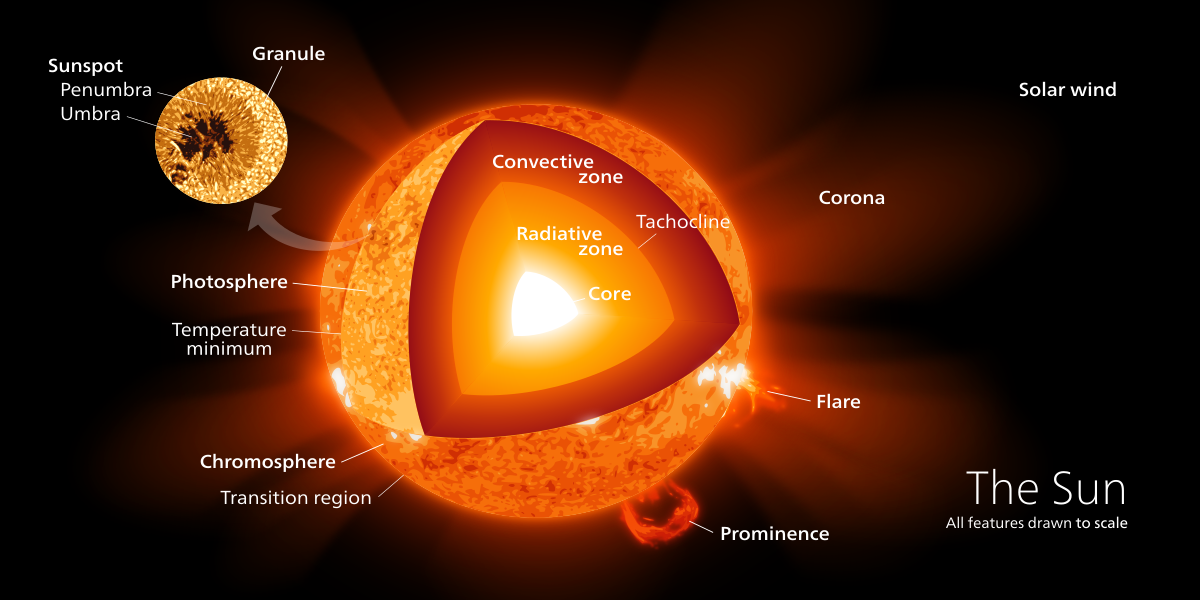
\includegraphics[width=0.8\textwidth]{graphics/solar_system_abundances/sun_structure}
    \caption{The structure of the Sun. Credit: Kelvinsong via \href{https://en.wikipedia.org/wiki/Sun}{Wikipedia}.}
    \label{fig:Sun_structure}
\end{figure}
Since the Sun contains the majority of the Solar System's mass, it is reasonable to assume that this celestial body also represents well the Solar System's composition. Figure~\ref{fig:Sun_structure} shows an artistic rendering of the structure of the Sun. The Sun's core extends to about a quarter of its radius and is the main nuclear engine that fuses hydrogen to helium at a temperature of around $16\times10^{6}$\,K.\footnote{Temperatures in astrophysics are often written as $T_x = y$. In this case, the actual temperature would be $y\times10^{x}$\,K. For the core of the Sun we could write the temperature thus as $T_{10} = 1.6$.} The solar core is not convectively connected to the outer layers, thus energy is mainly transported by radiative transfer. The photosphere, which is the visible part of the Sun, is at a temperature of around $5800$\,K. The atmosphere of the Sun has a minimum temperature of around 4100\,K about 500\,km above the photosphere. It consists of the chromosphere which lays above the photosphere and the solar corona that extends from the chromosphere out into space. At higher altitudes the temperature of the corona increases and reaches temperatures in excess of $10^6$\,K. How such high temperatures can be reached in the solar corona is still unclear.

\morebox{Wien's displacement law}{states that the radiation curve of a black-body has it's peak at different wavelengths depending on the temperature. For a given temperature, the peak wavelength can be calculated as:
\begin{equation}
    \lambda_\tn{max} = \frac{b}{T}
\end{equation}
Here, $T$ is the temperature in kelvin and $b = 2.898 \times 10^{-3}$ m$\cdot$K. Plugging in the photosphere temperature, we can calculate a peak wavelength at 500\,nm, which is the color green in the visible part of the electromagnetic spectrum.}


\subsection{Spectroscopy and Absorption Spectra}

\begin{figure}[tb]
    \centering
    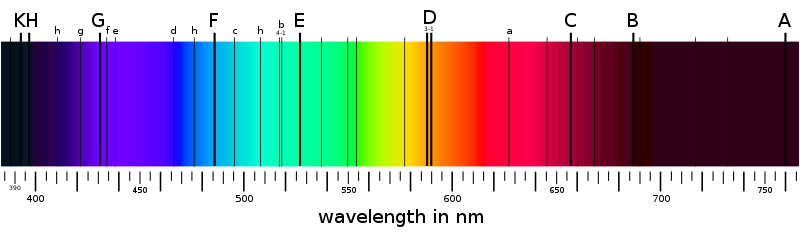
\includegraphics[width=0.8\textwidth]{graphics/solar_system_abundances/fraunhofer_lines_800px}
    \caption{The solar spectrum broken up into its components. Credit: \href{https://en.wikipedia.org/wiki/Fraunhofer_lines}{Wikipedia}.}
    \label{fig:fraunhofer_lines}
\end{figure}
In order to determine the composition of the Sun from the electromagnetic spectrum it radiates, astronomers use a technique called stellar spectroscopy. Using a prism or grating the light from the Sun is dispersed into its individual colors. Figure~\ref{fig:fraunhofer_lines} shows the electromagnetic spectrum of the Sun between 380\,nm and 710\,nm. Clearly visible are dark spectral absorption lines, so-called Fraunhofer lines named after Joseph von Fraunhofer who discovered, studied, and described them in 1814.

These absorption lines are fingerprints of the Sun's elemental composition. The dark lines form since photons coming out of the Sun are absorbed in the photosphere by atoms. The absorbed photons are subsequently re-emitted, however, this re-emission is not directed. Thus, the area of the spectrum that the original photon was absorbed in appears darker. For example, the double lines labeled ``D'' in Figure~\ref{fig:fraunhofer_lines} are a feature of the sodium absorption lines.


\subsection{Stellar Abundances} \label{sec:solar_abundances:sun:stellar_abundances}

In order to interpret the Fraunhofer lines observed from the Sun with respect to its elemental composition, many physical parameters and models must be known. Here we give a brief overview of these modeling efforts. Further details can be found in two great reviews on determining the Sun's elemental composition by \citet{asplund09} and \citet{allende-prieto16}.

To determine the composition of the Sun two closely related conditions must be understood: (1) line formation and (2) the stellar atmosphere. These two fields include physics from several disciplines, namely fluid dynamics, statistical mechanics, and thermodynamics. To understand line formation the atomic parameters and stellar conditions, such as the opacity, need to be known. To model stellar atmospheres on the other hand we need to know the energy radiated through the atmosphere, the surface gravity, and the chemical composition. Note that the chemical composition is on one hand what we would like to determine from these observations, however it is also an integral part of the stellar atmospheric model. The chemical composition has thus to be determined in an iterative process. For a given set of interest, especially the amount of energy radiated through it, its surface gravity, and its chemical composition. Note that the chemical composition, which is what we would like to find, must be known in order to model the stellar atmosphere. Determining the composition of the Sun from observations is thus an iterative process. For a given model atmosphere and determined atomic and molecular lines and continuum opacities, so-called spectra synthesis codes can be used to predict the spectrum of the model star with all its absorption lines. These spectra are then compared to observations. If different, the parameters, especially the chemical composition is updated with better values and the models are run again. The chemical composition of the star is found when model and observations agree.




\subsubsection{Photospheric Abundances}

The solar photosphere (see Figure~\ref{fig:Sun_structure}) is the part of the Sun that we can actually see. Spectroscopy of the photosphere is thus generally used to model the solar abundances. With a temperature between 4500\,K and 6000\,K and an effective temperature of around 5800\,K no molecules can form in the photosphere and thus only atoms are expected to contribute to its absorption lines. Furthermore, the densities of the chromosphere and corona above the photosphere are so low that they do not influence the absorption lines observed from the photosphere.

The present-day solar photosphere composition is slightly different from the initial Solar System abundance, i.e., the abundance that is representative of the homogeneous solar nebula. One difference of course is for radioactive nuclides that have decayed over the last 4.567\,Ga since the beginning of the Solar System. Furthermore, thermal diffusion, gravitational settling, and radiative acceleration -- the three of which are often collectively referred to as diffusion -- also changed the photospheric composition over the past 4.567\,Ga. Corrections for these effects must thus be applied before comparing Solar System initial abundances, as e.g., measured in meteorites (see Section~\ref{sec:sol_abu_meteorites}) with photospheric measurements.

\subsubsection{Chromosphere \& Corona Observations}

The chromosphere and corona are the solar layers right above the photosphere. These layers are too thin for us to directly observe and can generally only be seen during a total solar eclipse. Since there is no homogeneous background irradiation for the chromosphere and corona in these cases, absorption spectra cannot be measured. Thus, the elemental composition of the solar atmosphere is determined by measuring emission spectra. Excited atoms fall back to their ground states at discreet energies. Such emission lines will show up as bright instead of dark lines when analyzed in a spectrograph. 

Temperatures as low as 4100K have been measured in the chromosphere. This allows for the existence of simple molecules, which complicates the determination of the spectral abundances since many more atomic transitions are suddenly available. Furthermore, the chromosphere has a fairly large temperature gradient which also complicates the models. 

Coronal abundances are difficult to determine. The extremely high temperatures of the coronal make it difficult to determine radiative transitions in the laboratory. A large part of the coronal emission lines are furthermore in the \ac{uv} and \ac{euv}, thus can not be detected from Earth due to the atmosphere. Spacecrafts such as \ac{soho} have been used to determine the elemental composition of the solar corona.



\subsubsection{Solar Wind \label{sec:solar_abus:solar_wind}}

\begin{figure}[bt]
    \begin{subfigure}{0.470209674\textwidth}
        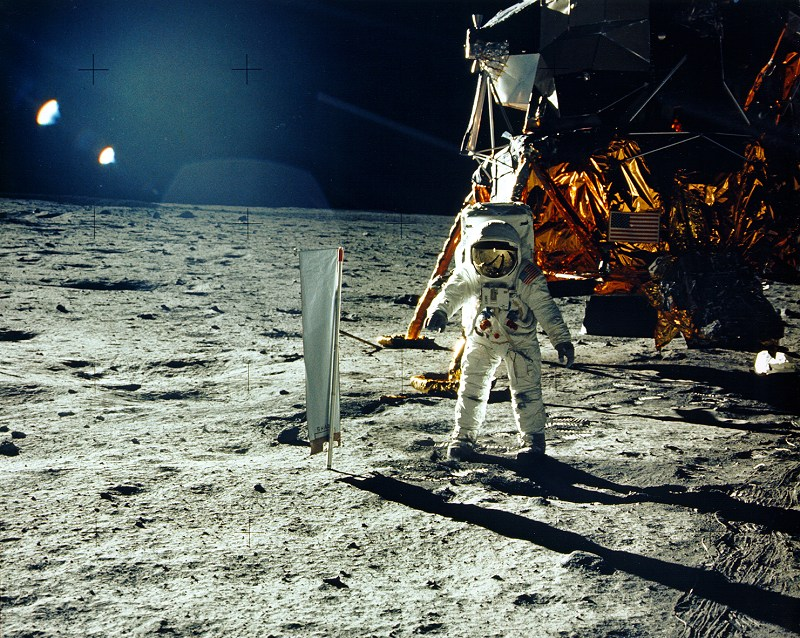
\includegraphics[width=\textwidth]{graphics/solar_system_abundances/apollo11_aldrin_solar_sail}
        \caption{Buzz Aldrin standing next to the solar sail during the Apollo 11 mission.}
        \label{fig:solar_wind_catcher_experiments:solar_sail}
    \end{subfigure}
    \begin{subfigure}{0.529790326\textwidth}
        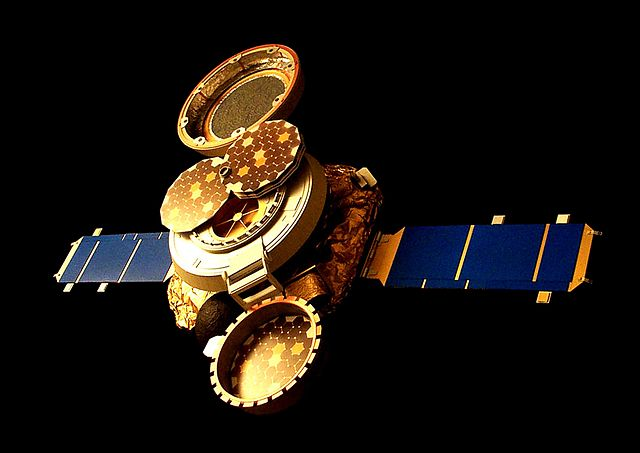
\includegraphics[width=\textwidth]{graphics/solar_system_abundances/genesis_spacecraft}
        \caption{Artist conception of the Genesis spacecraft with unfolded collectors.}
        \label{fig:solar_wind_catcher_experiments:genesis}
    \end{subfigure}
    \caption{The two types of solar wind catcher experiments that have been used to determine the composition of the Sun. Credit: NASA}
    \label{fig:solar_wind_catcher_experiments}
\end{figure}

Mass ejections such as prominences and flares (see Figure~\ref{fig:Sun_structure}) are the origin of the solar wind that penetrates the whole Solar System. The interaction of the solar wind with the Earth's magnetic field can, e.g., be seen as aurorae (borealis and australis), also known as the northern and southern lights. The solar wind consists to 98\% of protons (charged hydrogen particles). The other 2\% is mainly charged helium nuclei and a minute amount of heavier particles. This however means that the solar wind does carry some part of the Sun's composition out through the solar system.

While the solar wind cannot be measured on Earth, bodies without an atmosphere such as the Moon are constantly struck by solar wind. During the Apollo missions to the Moon, astronauts carried a solar sail, which was aluminum foil mounted on a pole in order to capture solar wind during their stay on the Moon. Figure~\ref{fig:solar_wind_catcher_experiments:solar_sail} shows Apollo 11 astronaut Buzz Aldrin standing next to the solar sail. While valuable measurements were done using solar sails flown on Apollo missions, the total exposure time of the aluminum foil was very limited, i.e., only up to a few days each. Thus, only little material was captured which resulted in significant analytical uncertainties when measuring the captured content.

In 2001, NASA launched the Genesis spacecraft which was parked on a Lagrange point L$_1$.\footnote{For more information, see \url{https://en.wikipedia.org/wiki/Lagrangian_point}} L$_1$ is a gravitationally semi-stable place in space in between the Sun and the Earth. Genesis exposed its collectors (Figure~\ref{fig:solar_wind_catcher_experiments:genesis}) to the solar wind for a total of 850\,d before returning to Earth. In order to avoid any contamination with terrestrial material, NASA's plan was for Genesis to re-enter the Earth's atmosphere, deploy its drogue parachute, and then capture the capsule mid-air using a helicopter with a long hook. The deployment mechanism for the parachute was connected to an accelerometer, which was unfortunately built backwards into the spacecraft. This resulted in the accelerometer measuring the acceleration with the wrong sign, thus never triggering the software to release the parachute. Needless to say that the ``landing'' of Genesis took place at a terminal velocity of around 86\,m\,s$^{-1}$ (190\,mph). This broke open the collector container and all collectors were significantly contaminated with material from the Utah dessert. Nevertheless, all main objectives of Genesis could still be achieved by meticulously cleaning and puzzling the collector array back together, a process that took several years.


\section{Meteorites}\label{sec:sol_abu_meteorites}

Meteorites are rocks that originated in the Solar System and fell to Earth as meteors. They are either finds, meaning that they were found during searches, or falls, meaning that they were found after observing the meteor in the sky. Meteorites could have previously been part of another planet, e.g., Mars, part of the Moon, or, most often, part of an asteroid. Thousands of these rocks have been analyzed, and they are generally classified into various different groups. The two major groups these rocks belong to relate them to their origin; they were either part of a differentiated or an undifferentiated parent body. A differentiated Solar System body has at some point in its history gotten hot enough in order to be completely or partially molten. This separated the metal-loving (siderophile) from the silicate loving (lithophile) elements. The Earth for example is a differentiated body with an iron, nickel core at the center and a silicate mantel around it. Meteorites from undifferentiated bodies, called chondrites, still contain the metal and silicate in the same phases, i.e., they have never gotten hot enough to differentiate. 

In order to determine the initial Solar System composition by analyzing meteorites, samples that have never been altered throughout its history are of special interest. These meteorites are called primitive. The most primitive subgroup of the chondrites are the carbonaceous chondrites, which have generally not even been heated enough in order to destroy the mineral phases that originally condensed from the solar nebula.

Alterations different from heat, e.g., chemical alterations, can also influence the composition and thus primitiveness of a meteorite. Meteorites that have been the least altered with respect to their chemical and isotopic composition are carbonaceous chondrites that are similar to the Ivuna meteorite, which is the type specimen for this group. The name of this chondrite group is thus abbreviated CI chondrites. The Orgueil meteorite, a CI chondrite, represents the best studied sample for the Solar System initial abundance. This rock fell on May 14, 1864 just after 8pm local time near Orgueil, a town in southern France. Samples were recovered immediately, totaling 14\,kg of material. Meteorite falls have the advantage that they did not spend any significant amounts of time exposed to the weather on Earth, thus they do not show any terrestrial alteration either. 

To determine the composition of meteorites, their material is usually homogenized and then analyzed using a mass spectrometery. Depending on the element of interest sample material is atomized and ionized. These ions are then separated by mass-over-charge in a mass analyzer. This allows for precise determination of their elemental and isotopic composition.

\morebox{Stardust}{Some primitive meteorites contain micrometer sized grains that in fact did not form in the Solar System at all but rather represent bona-fide stardust grains. These stardust grains formed in the outflow of dying stars, were transported through the \ac{ism}, and then incorportated into meteorite parent bodies during their formation. We will discuss stardust grains in more detail later since these samples allow us to directly probe the processes in which elements are created.}



\section{The Composition of the Solar System}

While CI chondrites seem to be primitive Solar System objects, their total mass is represents only a tiny fraction of the total mass of the Solar System. Photosphere observations on the other hand are associated with larger measurement uncertainties and require modeling of the physical processes underlying the formation of absorption spectra. The question thus arises on how the composition of the Solar System can best be determined.

\subsection{Comparing CI chondrites and the Photosphere}

\begin{figure}[bt] \centering
    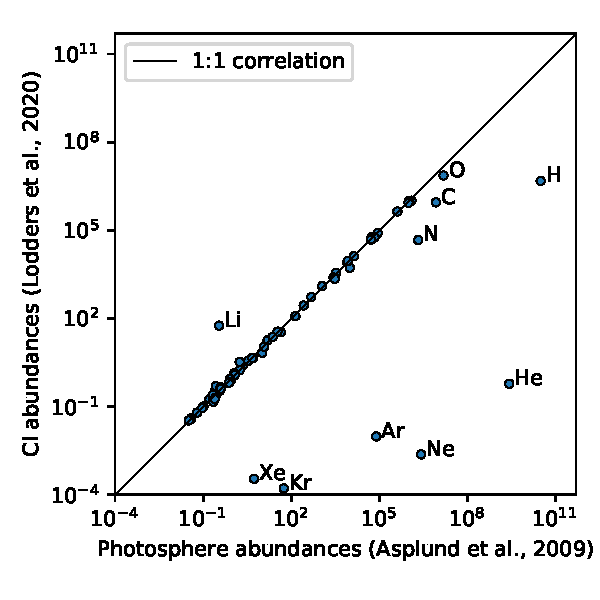
\includegraphics[width=0.5\textwidth]{graphics/solar_system_abundances/solar_photosphere_ci_abundances_correlation}
    \caption{Comparison of solar photosphere measurements \citep{asplund09} and the composition of CI meteorites \citep{lodders20}. Elements that do not lie close to the 1:1 correlation line are labeled.}
    \label{fig:solar_photosphere_ci_comparison}
\end{figure}
Figure~\ref{fig:solar_photosphere_ci_comparison} shows the comparison of the photosphere measurements reported in \citet{asplund09} with the CI chondrite measurements reported in \citet{lodders20}. Most elements lie perfectly on the 1:1 correlation indicated in black in the figure, which spans a total of around 12 orders of magnitude. However, there are some very notable deviations that require further discussion.

\paragraph{Lithium} is the only element that is more abundant in CI chondrites than in the Sun. In the Sun, lithium diffuses effectively. Since it is destroyed during the nuclear reactions taking place in the stellar core, the overall abundance of lithium is expected to be depleted when compared to the bulk Solar System.

\paragraph{The noble gases} helium, neon, argon, krypton, and xenon are all very volatile and are thus heavily depleted in meteorites, i.e., they never effectively condensed into the rocky material when meteorite parent bodies formed. The bulk Solar System helium abundance can fortunately be derived from helioseismology via observations of the Sun and is not highly model dependent. Various techniques have been used to determine the composition of the other noble gases. One of the most accurate methods to-date is the analysis of solar wind in the Genesis collectors, see page~\pageref{sec:solar_abus:solar_wind}.

\paragraph{Hydrogen} is also a highly volatile element and thus does not effectively condense into meteorite parent bodies. Hydrogen thus needs to be measured in the Sun by model comparison. The hydrogen mass is insensitive to the Z/X composition of the Sun, which results in an accurate determination of the hydrogen mass fraction X.

\paragraph{Carbon, nitrogen, and oxygen} are prominent atoms that form volatile molecules, e.g., CO, CO$_2$, N$_2$, and O$_2$. Thus, these elements are expected to be depleted in rocky materials. While these elements can all be measured in the solar photosphere, model improvements resulted in significant changes over time in their abundances.

\subsection{Solar System Elemental Abundances}

\begin{figure}[bt] \centering
    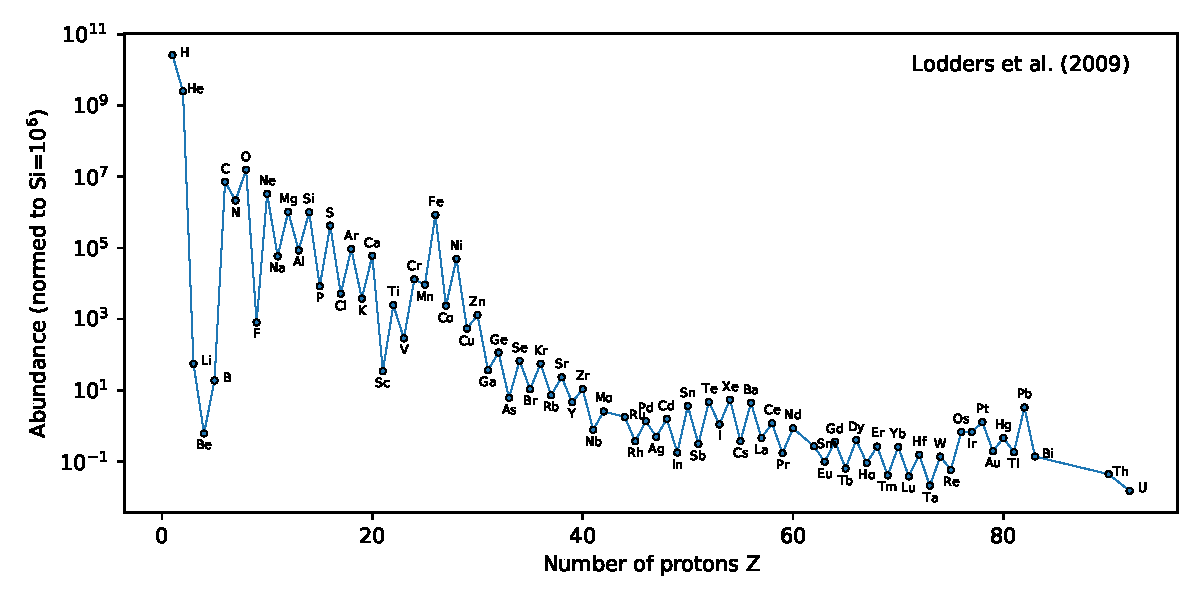
\includegraphics[width=\textwidth]{graphics/solar_system_abundances/solar_system_abundances}
    \caption{Solar System initial abundances for all elements \citep{lodders09}.}
    \label{fig:solar_system_abundances}
\end{figure}
Figure~\ref{fig:solar_system_abundances} shows the elemental abundances of the solar nebula. Clearly, hydrogen and helium are the most abundant elements. Furthermore, we can see a clear peak around carbon, oxygen, and neon. These elements are made in most stars and thus reach such high abundances. There is also a clear peak at the iron isotopic composition. This is due to the fact that in this region, the binding energy per nucleon is the highest across all elements. That means that energy can be gained by fusing nuclides together up to iron. Past iron this does not happen anymore, thus the abundances of all heavier nuclides drop significantly.

Another striking feature of the abundance curve in Figure~\ref{fig:solar_system_abundances} is the clear zigzag pattern. This pattern is due to the fact that even nuclei, i.e., nuclei with an even number of nucleons (protons and neutrons), have a higher binding energy than odd nuclei and are thus more stable. 


\subsection{Solar System Isotopic Abundances}

So far we have mostly discussed the abundance of the elements in the Solar System. Just as important is the abundance of the isotopes, which can be derived from CI chondrites with high precision. Atomic line differences of individual isotopes are generally too small in order to derive useful isotopic abundances from solar observations. Let us briefly discuss the origin of a few important isotopes cannot easily be derived from CI chondrites.

\paragraph{Deuterium and \ex{3}He} are both highly volatile, thus cannot be measured in CI chondrites, and have been significantly changed in the Sun. In its early stage the Sun underwent deuterium burning, essentially leaving it deuterium free at this point. This burning also produced \ex{3}He and thus changed its abundance in the Sun. The exact D/H ratio in the Solar System is still an active matter of research. Good analogues to determine this ratio are the atmosphere of Jupiter which consists mainly of the gaseous material that the solar nebula was made of, and in comets. Certain, so-called Kuiper-belt comets formed far out in the Solar System beyond the snow-line, which is the area of the solar nebula beyond which water only appears in solid form. These comets thus trapped the original D/H composition. For the early Solar System \ex{3}He/\ex{4}He ratio, the value for Jupiter's atmosphere is generally adopted.

\paragraph{Carbon, nitrogen, and oxygen} are all very volatile. While the carbon isotopic composition in the Solar System is not very variable across different types of meteorites, the nitrogen and oxygen isotopic composition vary widely. To measure these isotopes in solar wind was one of the main objectives of the Genesis mission. After significant cleaning of these collectors, the solar oxygen and nitrogen isotopic composition have finally been determined by \citet{mckeegan11} and \citet{marty11}, respectively.

\paragraph{Noble gases} are also volatile. As discussed before, their elemental and isotopic abundances were determined using the solar wind collectors on board the Genesis spacecraft. A detailed review of this work can be found in \citet{heber09}.



\subsection{Preview on the Origin of Elements and Isotopes}

So far we have only briefly discussed the major features visible in the Solar System abundance pattern (Figure~\ref{fig:solar_system_abundances}). We will look into a lot more details on how individual elements and groups formed later on. The production of elements and their isotopes takes place in a process called nucleosynthesis. A brief overview of these processes is given below.

All hdrogen and helium in universe formed right after the Big Bang in a process called \acl{bbn}. The majority of all heavier elements were subsequently formed in stars. Elements up to the iron peak formed mainly in massive stars by nuclear fusion reactions. As discussed before, the binding energy per nucleon is the highest at iron and thus fusion reactions beyond this region are not energetically favorable. Thus, other processes must take over. 

Most isotopes beyond iron are formed by neutron-capture reactions. Since neutrons are not electrically charged, they do not see the Coulomb barrier of a positively charged nucleus and can thus be more effectively added to it. Neutron addition takes place until the nucleus becomes unstable. Unstable, neutron-rich nuclei decay generally via $\beta^{-}$-decay to the next stable isobar, which has one proton more and one neutron less. Proton-rich nuclei, e.g., \ex{92}Mo, cannot form by neutron capture and various processes and locations for their formation are actively being discussed in the astrophysics community.

About half the elements beyond iron formed in the so called \ac{sproc}, in which the $\beta^{-}$ decay to the stable isobar generally happens faster than another neutron can be captured. This way however, only elements up to bismuth can be made. Heavier elements, e.g., actinides such as thorium and uranium, cannot be formed in the \ac{sproc}. Rapid capture of neutrons, the so-called \ac{rproc}, must thus be invoked to explain their existence.



\section{Other Stars}

While we have Solar System samples, i.e., CI chondrites, to determine the composition of the solar nebula and thus the Sun precisely, representative rocks of other stars are not available in the Solar System. However, the light of other star still reaches us, i.e., we can see their photosphere and apply the same spectroscopic techniques to determine their elemental composition. 

As discussed in Section~\ref{sec:solar_abundances:sun:stellar_abundances}, to determine the abundances of observed other stars, the stellar atmosphere must be modeled. For this, the size and mass of the star must be known, which is not always simple to determine from observations. Recent massive surveys such as the Sloan Digital Sky Survey\footnote{\url{https://www.sdss.org/}} and the Gaia mission\footnote{\url{https://sci.esa.int/web/gaia/}} have made it possible to determine the elemental composition of many more stars. An overview of existing database can, e.g., be found in \citet{allende-prieto16}. It turns out that the solar neighborhood is a diverse place \citep[see, e.g.,][]{bensby14} and still leaves us for the time being with many open question on the origin of its elements and isotopes.

\section{Reading}

A great reading to further dive into the topic of solar abundances is the recent review by \citet{lodders20}.\footnote{At the time of this writing, the download of the document as a \ac{pdfdoc} file did not succeed. You can also find this article on \href{https://arxiv.org/abs/1912.00844}{ArXiV}.} Some questions and points of discussions for this paper are:
\begin{itemize}
    \item Why are meteoritic measurements normalized to a silicon abundance of $10^6$ while astronomical observations are generally given in \ac{dex} noramlized such that the abundance of hydrogen is equal to 12?
    \item Why can elemental abundances with much higher precision in CI chondrites than in the Sun's photosphere?
    \item Why does aqueous alteration not affect the chemical composition of CI chondrites?
    \item Explain from a nuclear physics point of view why there is no deuterium in the Sun.
    \item Why is it so difficult to determine certain elemental and isotopic abundances, e.g., noble gases and the D/H ratio of the Solar System?
    \item What are the difficulties that one encounters when analyzing meteorites by mass spectrometry?
    \item Why can carbon, oxygen, and nitrogen not be determined when analyzing meteorites?
\end{itemize}
% %!TEX root = origin_elements_lecture_notes.tex

\chapter{Big Bang Nucleosynthesis}

In order to understand primordial / \acf{bbn}, we need to first look at some fundamental observations that define cosmology. In addition, we also need to introduce the standard model of cosmology. Note that this is only a very brief introduction into a topic that could be a whole course by itself.

\section{Fundamental Cosmological Observations}

\subsection{Olbers' paradox}

One of the most fundamental observations that goes back to Kepler (1610), Halley (1721), de Cheseaux (1744), and is today known as Olbers' (1823) paradox is the fact that the night sky is dark. If one assumes an infinite, homogeneous space filled with stars, this space would appear infinitely bright to the observer on Earth. The apparent luminosity of a star can be described as
\begin{equation}\label{eqn:bbn:relative_luminosity}
    l = \frac{L}{4 \pi r^{2}} \propto r^{-2},
\end{equation}
where $L$ is the star's luminosity and $r$ its distance from Earth. Assuming a density of stars $n$, a spherical shell of thickness $dr$ at distance $r$ from Earth would contain
\begin{equation}
    dN = 4 \pi n r^2 dr \propto r^2
\end{equation}
stars. The total energy density of all stars for an observer can thus be calculated as
\begin{equation}\label{eqn:bbn:total_energy_density}
    \varepsilon_s = \int_0^{\infty} \frac{L}{4\pi r^2} dN = nL \int_{0}^{\infty} dr.
\end{equation}
In contrast to our experience this integral is divergent, thus the night sky should be infinitely bright. 

This paradox cannot be simply solved by assuming absorption of light in the interstellar medium, e.g., by dust. The energy from all stars would over time heat up this dust until it radiates as bright as the stars themselves. One factor that slightly helps is that stars will overlap with each other. You can picture this scenario however like standing in a dense forest where, as far as you can see, every line of sites terminates in a tree trunk. For the universe this would mean that every line of sight will terminate at the surface of a star. Stars cover each other, so the night sky would not seem infinitely bright but homogeneously about as bright as the Sun. This still does not agree with our experience.

The solution to the paradox lies in the fact that the universe is expanding. The wavelength of the light that arrives expands along with the universe and is thus shifted to the red (Doppler shift). The result is that the relative luminosity, as given in equation \eqref{eqn:bbn:relative_luminosity}, is in fact $l\propto r^{-3}$. Plugging this into equation~\eqref{eqn:bbn:relative_luminosity} results in the integral converging. In addition, there the universe has a horizon at distance
\begin{equation}
    R \simeq ct.
\end{equation}
Here, $c$ is the speed of light and $t$ the approximate age of the universe. The visible part of space and thus the energy density become finite.

\infobox{Doppler effect}{Let us assume that a source emits an electromagnetic wave with wavelength $\lambda_s$. An observer that moves with a velocity $\vec{v}$ with respect to that source will register a shifted frequency $\lambda_r$. For light, and considering special relativity, this effect will result in a blueshift if the observer moves towards the source and in a redshift if the observer moves away from the source. For two objects that move directly towards or away from each other, the relativistic Doppler shift for light can be written as
\begin{equation}\label{eqn:bbn:relativistic_doppler_shift}
    \lambda_r = \sqrt{\frac{1+\beta}{1-\beta}} \lambda_s,
\end{equation}
where $\beta = v/c$, i.e., the speed of the observer $v$ with respect to the speed of light $c$. Sources moving away from each other hereby have a postive velocity ($\beta > 0$), sources moving towards each other a negative one ($\beta < 0$).}

\subsection{Hubble's Law}

\begin{figure}[tb]
    \centering
    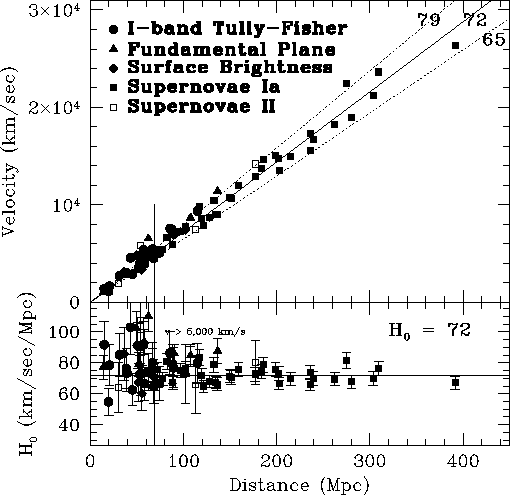
\includegraphics[width=0.5\textwidth]{graphics/bbn/hubble_diagram}
    \caption{Hubble diagram of velocity (top) and value of $H_0$ (bottom) as a function of distance. \cite{freedman01}, \copyright\ 2001 The American Astronomical Society.} 
    \label{fig:bbn:hubble_diagram}
\end{figure}
The expansion of the universe can in fact be observed. Figure~\ref{fig:bbn:hubble_diagram} shows the Hubble diagram for many observations, taken from \citet{freedman01}. The diagram on top shows the velocity of objects relative to Earth as a function of their distance. Using the Doppler shift one can see that the velocity, which is away from the observer in this case, is proportional to the redshift of the object. Here, the distance is given in megaparsec, where 1\,\ac{pc} is approximately 3.26 light years. The linear relationship between velocity and distance (R) can be written as
\begin{equation}
    \left(\frac{\dot{R}}{R}\right)_0 = H_0 = \mathrm{constant}.
\end{equation}
The subscript zero hereby describes the present-day value of the constant. The constant $H_0$ is commonly called the Hubble constant and its value is about $H_0 = 70\,\mathrm{km}\,\mathrm{s}^{-1}\,\mathrm{Mpc}^{-1}$. Note that the Hubble constant is given in units of one over seconds. The reciprocal value of the $H_0$ thus defines a time, the so-called Hubble time. If the expansion of the universe is never accelerated, its age could be determined as
\begin{equation}
    t_0 \leq \frac{1}{H_0} = 1.4 \times 10^{10}\,\mathrm{a}.
\end{equation}

The distance of a galaxy is often expressed by its redshift. Let $\lambda$ be the wavelength sent out from the galaxy in question and $\lambda_0$ the wavelength received today. The redshift $z$ can then be written as
\begin{equation}\label{eqn:bbn:redshift}
    1+z = \frac{\lambda_0}{\lambda} = \frac{R_0}{R}.
\end{equation}
Here, $R$ is introduced as the so-called scale factor of the universe.

Since the universe consists of mass that interacts gravitationally with each other, we can define a deceleration parameter $q_0$ for the universe such that
\begin{equation}
    \label{eqn:bbn:decceleration}
    q_0 \equiv -\left(\frac{\ddot{R} R}{\dot{R}^2}\right) = - \frac{\ddot{R_0}}{R_0 H_0^2}.
\end{equation}


\subsection{Density of Matter}
By density one generally refers to the total energy density of all components (radiation, matter, and dark energy) divided by $c^2$. While radiation dominated in the early universe, matter or even dark energy dominates today. The total density of matter in the universe can be measured by determining the total mass of individual galaxies. An estimated density can thus be given as
\begin{equation}
    2 \times 10^{-31}\,\mathrm{g}\,\mathrm{cm}^{-2} \leq \rho_0 \leq 2\times10^{-30}\,\mathrm{g}\,\mathrm{cm}^{-2}.
\end{equation}

\morebox{Dark matter}{In 1933, Fritz Zwicky noticed that galactic cluster do not rotate as expected. By constraining the observed mass in the cluster and observing its rotation, Zwicky noticed that some matter was missing. He called this dark matter. Figure~\ref{fig:bbn:galactic_rotation} shows an example of the expected and observed rotation curves. From this and further observations we can derive that dark matter makes up around 85\% of all matter in the universe. Only 15\% of the matter in the universe consists of baryons, e.g., particles made up of quarks such as neutrons and protons.}
\begin{figure}[tb]
    \centering
    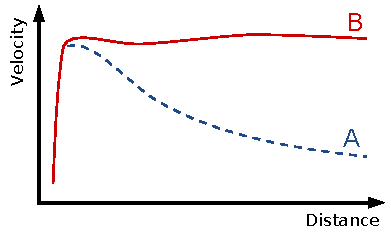
\includegraphics[width=0.45\textwidth]{graphics/bbn/galactic_rotation}
    \caption{Galactic rotation: Case A shows the expected behavior, case B the observed one. Credit: \href{https://en.wikipedia.org/wiki/Dark_matter}{Wikipedia}.}
    \label{fig:bbn:galactic_rotation}
\end{figure}



\subsection{Cosmic Microwave Background}

In the Big Bang model, the universe started from a very hot and dense state. One expected remnant of this state is a relic radiation that in fact was detected in 1965 by Arno Penzias and Robert Wilson \citep{penzias65}. The detection of this \ac{cmb} is one of the pillars supporting the Big Bang model to describe the origin of the universe. The origin of the \ac{cmb} will be discussed in further detail below.

The \ac{cmb} is a thermal blackbody radiation with a measured temperature of $2.72548 \pm 0.00057$\,K. The peak of this radiation is in the microwave range and cannot be observed from Earth. Space missions such as \href{https://map.gsfc.nasa.gov/}{\ac{wmap}} and \href{http://www.esa.int/Science_Exploration/Space_Science/Planck}{Planck} measured the \ac{cmb} in detail. A map of the \ac{cmb} is shown in Figure~\ref{fig:bbn:wmap_cmb}.
\begin{figure}[tb]
    \centering
    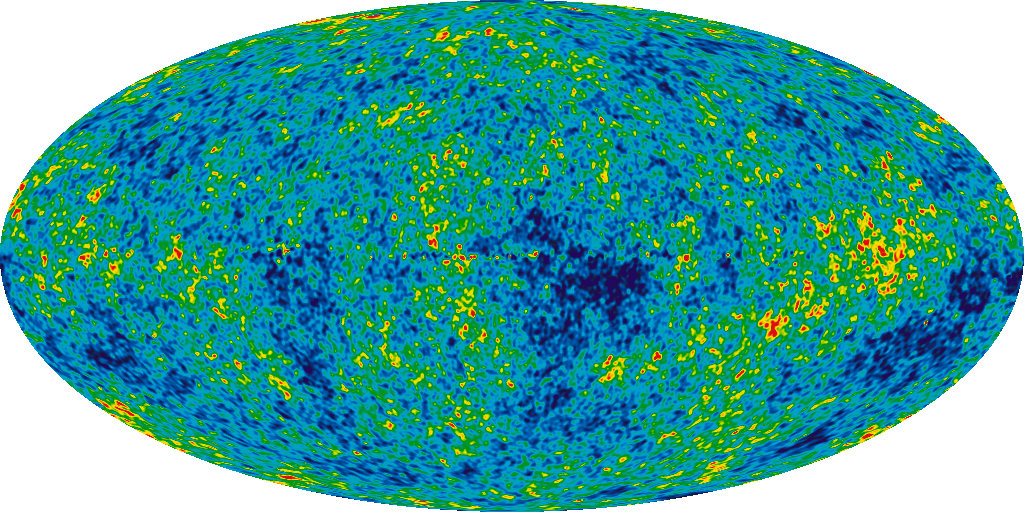
\includegraphics[width=0.75\textwidth]{graphics/bbn/wmap_cmb}
    \caption{\ac{wmap}'s image of the \ac{cmb}. Shown is averaged data from nine years of measurements. Credit: \href{https://map.gsfc.nasa.gov/media/121238/index.html}{NASA}.}
    \label{fig:bbn:wmap_cmb}
\end{figure}



\section{The Standard Model of Cosmology}

The standard model of cosmology describes the origin of the universe and its evolution based on one singular event: the Big Bang. With the Big Bang, space, time, and matter came into existence and the universe developed from its hot, dense state to the cold and transparent state we see today.

\subsection{Assumptions}\label{sec:bbn:standard_model:assumptions}

The standard model of cosmology is based on several key assumptions. Here we focus on the ones that are of importance to understand \ac{bbn}.

\begin{enumerate}
    \item The cosmological principle is valid. This states that the spatial distribution of matter in the universe in homogeneous and isotropic. \label{it:bbn:cosmological_principle}
    \item The overall charge in the universe is zero.
    \item The universe is made of matter and not of antimatter. This assumption in fact directly contradicts the cosmological principle (assumption \ref{it:bbn:cosmological_principle}) since it requires that there was an overabundance of baryons compared to antibaryons at the start of the universe, making it thus inhomogeneous. This overabundance of matter is to this date not fully explained and remains under active investigation.
    \item At temperature $T<10^{11}$\,K (approximately 10\,ms after the Big Bang), all heavy particles were annihilated and the density of the universe is defined by photons, neutrinos ($\nu$), electron and positrons ($\mathrm{e}^{\pm}$), and the remaining baryons.
\end{enumerate}


\subsection{Temperature and Density Evolution}

\begin{figure}[tb]
    \centering
    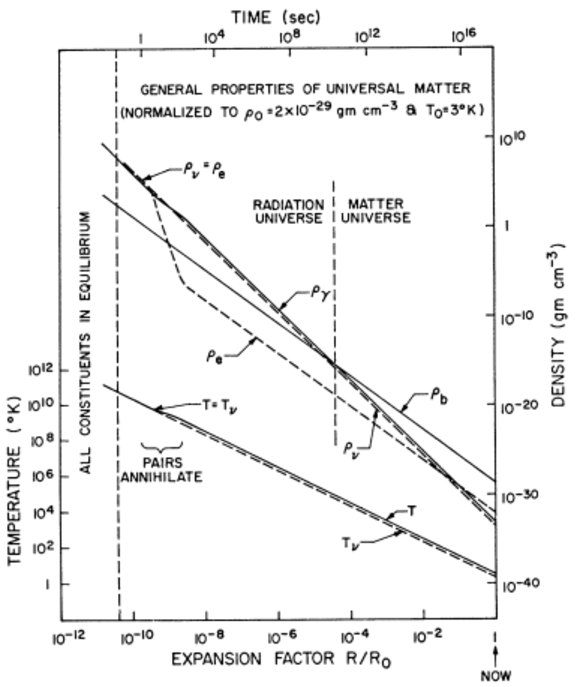
\includegraphics[width=0.6\textwidth]{graphics/bbn/wagoner67_fig1}
    \caption{The temperature and density evolution of the universe in the framework of the standard model of cosmology. Taken from \citet{wagoner67}. \copyright\ American Astronomical Society.}
    \label{fig:bbn:cosmology_phases}
\end{figure}
Figure~\ref{fig:bbn:cosmology_phases} shows the temperature and density evolution of the universe in the framework of the standard model of cosmology \citep{wagoner67}. The horizontal axis show the expansion factor $R/R_0$ as defined in equation \ref{eqn:bbn:redshift} on the bottom and the time since the Big Bang on the top. The vertical axes show the temperature (left) and the density (right). The standard model description starts at around 10\,ms with all constituents in equilibrium. \acl{bbn} sets in at a temperature of around $10^{9}$\,K. 



\section{Big Bang Nucleosynthesis}

\subsection{The Proton-to-Neutron Ratio}

In the beginning at a temperature of around $10^{11}$\,K (see Figure~\ref{fig:bbn:cosmology_phases}), the protons and neutrons are in thermodynamic equilibrium. Statistical mechanics shows that the energy of such a system can be expressed using the Boltzmann distribution for the individual states. This can be used to express the ratio of the number of protons to the number of neutrons in equilibrium conditions as
\begin{equation}\label{eqn:bbn:td_equilibrium_number_ratios}
    \left(\frac{n_\mathrm{p}}{n_\mathrm{n}}\right)_\mathrm{eq} 
        = \frac{\lambda_\mathrm{np}}{\lambda_\mathrm{pn}}
        = \exp\left(\frac{(m_\mathrm{n} - m_\mathrm{p})c^2}{kT}\right)
        = \exp\left(\frac{1.501}{T_{10}}\right).
\end{equation}
Here, $\lambda_\mathrm{np}$ and $\lambda_\mathrm{pn}$ are the reaction rates to turn a neutron into proton and vice verse, respectively. For $T\rightarrow\infty$ protons and neutrons will have equal abundances. At lower temperatures however, protons will become more abundant. 

We can rewrite equation~\eqref{eqn:bbn:td_equilibrium_number_ratios} to express the mass fractions of neutrons in equilibrium as
\begin{equation}
    X_\mathrm{n,eq} = \left(\frac{n_\mathrm{n}}{n_\mathrm{p} + n_\mathrm{n}}\right)_\mathrm{eq}
    = \frac{1}{(n_\mathrm{p} / n_\mathrm{n})_\mathrm{eq} + 1}
    = \frac{\lambda_\mathrm{pn}}{\lambda_\mathrm{pn} + \lambda_\mathrm{np}}.
\end{equation}


The nucleons react with each other via the weak force and the following reactions are possible:
\begin{eqnarray}
    \mathrm{n} + \nu &\longleftrightarrow& \mathrm{p} + \mathrm{e}^{-} \\
    \mathrm{n} + \mathrm{e}^{+} &\longleftrightarrow& \mathrm{p} + \bar{\nu} \\
    \mathrm{n} &\longrightarrow& \mathrm{p} + \mathrm{e}^{-} + \bar{\nu} \label{eqn:bbn:neutron_decay_reaction}
\end{eqnarray}
Reaction \eqref{eqn:bbn:neutron_decay_reaction} is the free decay of neutrons and has a half-life of 610\,s. This reaction can thus be neglected at the beginning since it is very long compared to all other reactions. The neutron mass fraction over time follows thus the differential equation
\begin{equation}
    \frac{d}{dt}X_\mathrm{n}(t) = -\lambda_\mathrm{np}(t)X_\mathrm{n}(t) + \lambda_\mathrm{pn}(t)[1-X_\mathrm{n}(t)].
\end{equation}
With decreasing temperature the reaction rates $\lambda_\mathrm{np}$ and $\lambda_\mathrm{pn}$ go rapidly towards zero such that after around 10\,s the proton to neutron ratio is frozen in place. Calculating reaction rate values, e.g., as in \citet{peebles66apj}, the neutron mass fraction at freezeout (when the reaction rates $\lambda_\mathrm{np}$ and $\lambda_\mathrm{pn}$ go to zero) is
\begin{equation}
    X_\mathrm{n,freeze} = 0.164.
\end{equation}
From this time on, the only reaction taking place is free neutron decay, see reaction~\eqref{eqn:bbn:neutron_decay_reaction}. Since the half-life of neutrons is fairly short, they must rapidly after the freezeout be captured as part of atomic nuclei in order to not decay away.


\subsection{Nucleosynthesis of Deuterium}

Deuterium has a mass of $m_\mathrm{D} = 1875.612928$\,MeV, while a proton and neutron have masses of $m_\mathrm{p} = 938.272088$\,MeV and $m_\mathrm{n} = 939.565421$\,MeV (see info box below for an explanation of measurements in eV).  
\begin{table}[b]  % since info boxes are in tabular environments...
\infobox{Measurements in eV}{In nuclear physics, masses are often expressed in mega electronvolts or MeV, which is technically not a mass but an energy. The mass of the particle is related to its energy via Einstein's equation $m=E/c^2$. Thus, energy and mass are directly related with $c$, the speed of light, as a proportionality constant. Similarly we can write the momentum of a particle as $\vec{p} = E \vec{c}^{-1}$ and the temperature of a system as $T = E k_B^{-1}$. Here, $k_B$ is the Boltzmann constant. Since mass, momentum, and temperature are related to energy via constants, these quantities are often expressed as energies.}
\end{table}
Deuterium, an isotope of hydrogen (\ex{2}H), consists of one proton and one neutron. However, summing the mass of one proton and one neutron results in a mass that is $\Delta m = 2.22$\,MeV larger than the mass of deuterium. This so-called mass defect defines the binding energy of deuterium and is the reason why energy is released when a proton and neutron are fused together. In chemistry this would be called an exothermic reaction. It can be written as
\begin{equation}\label{eqn:bbn:deuterium_formation_reaction}
    \mathrm{p} + \mathrm{n} \longrightarrow \mathrm{D} + \gamma.
\end{equation}
\begin{figure}[tb]
    \centering
    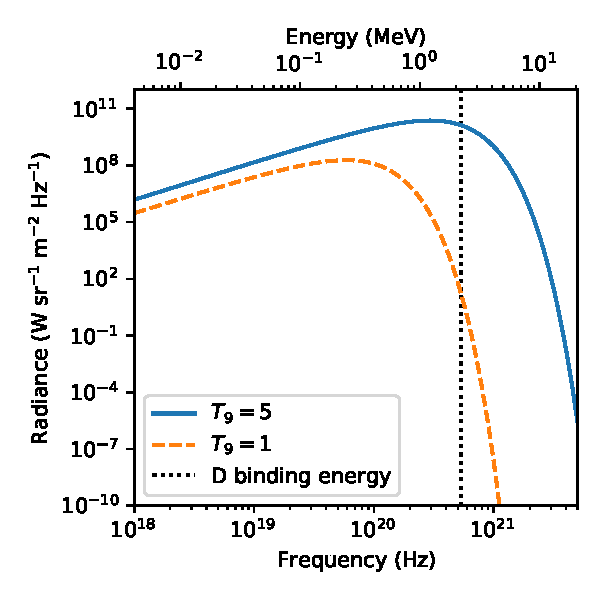
\includegraphics[width=0.5\textwidth]{graphics/bbn/planck_radiation_bbn}
    \caption{Spectral energy of black body radiation at the temperature when neutrons and protons are in equilibrium ($T_{9} \approx 5$) and when deuterium fusion can start ($T_{9}\approx1$). Prior to this temperature, the photon energies are too high and destroy newly formed deuterium effectively.}
    \label{fig:bbn:planck_radiation_deuterium_fusion}
\end{figure}

At the time when $n_\mathrm{p}/n_\mathrm{n}$ is frozen, the temperature of the universe is still $T\approx 5\times 10^{9}$\,K. Any deuterium that forms at this temperature is effectively destroyed right away again, since many photons have enough energy to dissociate the binding energy of 2.22\,MeV. Figure~\ref{fig:bbn:planck_radiation_deuterium_fusion} shows the spectral energy of a blackbody at this high temperature as a function of the frequency of the photons (bottom axis) and as function of their energy in MeV (top axis). The black, dashed line shows the deuterium binding energy. Note that both axes of the figure are logarithmic. Clearly, at $T_9 = 5$ many photons still have high enough energies. The universe thus first needs to cool down below $T_9 \approx 1$ before deuterium can effectively form. 

The exact temperatures, as just described, do not only depend on the temperature but also on the abundance of photons. Furthermore, the temperature is directly related to the density of the universe. Figure~\ref{fig:bbn:planck_radiation_deuterium_fusion} thus only gives a relative insight into the dissociation of deuterium. More detailed calculations can be found in the literature, e.g., in \citet{wagoner67}.

The drop in temperature of the universe from when proton and neutron abundances are frozen until deuterium can effectively form without being destroyed takes about 220\,s. During this time, the neutrons still undergo free decay. Using equation~\eqref{eqn:radioactive_decay} we can calculate that by the time deuterium fusion becomes significant, another $\sim20$\% of the neutrons decay.
This leaves behind a neutron fraction of
\begin{equation}
    X_n = 0.128
\end{equation}
at the start of \ac{bbn}.

\subsection{Nucleosynthesis of Helium}

Once deuterium has formed, more reactions can take place. Some of these reactions are:
\begin{eqnarray}
    \mathrm{D} + \mathrm{D} &\longleftrightarrow& ^3\mathrm{He} + \mathrm{n} \\
    \mathrm{T} + \mathrm{p} &\longleftrightarrow& ^3\mathrm{He} + \mathrm{n} \\
    \mathrm{T} + \mathrm{D} &\longleftrightarrow& ^4\mathrm{He} + \mathrm{n} \\
    \mathrm{p} + \mathrm{D} &\longleftrightarrow& ^3\mathrm{He} + \gamma \\
    \mathrm{n} + \mathrm{D} &\longleftrightarrow& \mathrm{T} + \gamma \\
    \mathrm{p} + \mathrm{T} &\longleftrightarrow& ^4\mathrm{He} + \gamma \\
    \mathrm{n} + {^3}\mathrm{He} &\longleftrightarrow& ^4\mathrm{He} + \gamma \\
    \mathrm{D} + \mathrm{D} &\longleftrightarrow& ^4\mathrm{He} + \gamma
\end{eqnarray}
Here, T is a tritium nucleus, another isotope of hydrogen with two neutrons (\ex{3}H). The reaction rates for these individual paths can be calculated, however, let us first estimate the dominant product of big bang nucleosynthesis. For deuterium above we determined a binding energy of 2.22\,MeV. Calculating the mass defect and thus the binding energy for \ex{3}He and \ex{4}He gives 6.70\,MeV and 27.3\,MeV, respectively. A better way to compare these binding energies is however to determine the binding energy per nucleon. For \ex{3}He and \ex{4}He these would be 2.23\,MeV per nucleon and 6.81\,MeV per nucleon. Thus, \ex{4}He is much favored to being produced. 

If we assume that all neutrons will be bound into \ex{4}He, a fairly accurate assumption as we will see further down, we can now predict the mass fraction of helium ($Y$) in the universe. After free decay of neutrons, we are left with $X_\mathrm{n} = 0.128$. Since \ex{4}He is roughly four times heavier than hydrogen, we can estimate the mass fraction of $^{4}$He as
\begin{equation}
    Y = \frac{4n_\mathrm{He}}{4n_\mathrm{He} + n_\mathrm{H}} 
        = \frac{2n_\mathrm{n}}{n_\mathrm{p} + n_\mathrm{n}}
        = \frac{2(n_\mathrm{n} / n_\mathrm{p})}{1+(n_\mathrm{n}/n_\mathrm{p})}
        = 0.23.
\end{equation}
This estimated value is in excellent agreement with the observed abundance of helium in the universe of about $1/4$ and is thus another robust pillar for the Big Bang model.


\subsection{Nucleosynthesis of heavier elements}

The highest binding energy per nucleon is found in the isotope \ex{62}Ni. However, several reasons contribute to the fact that \ac{bbn} cannot synthesize nuclides heavier than \ex{7}Li.

\begin{figure}[tb]
    \centering
    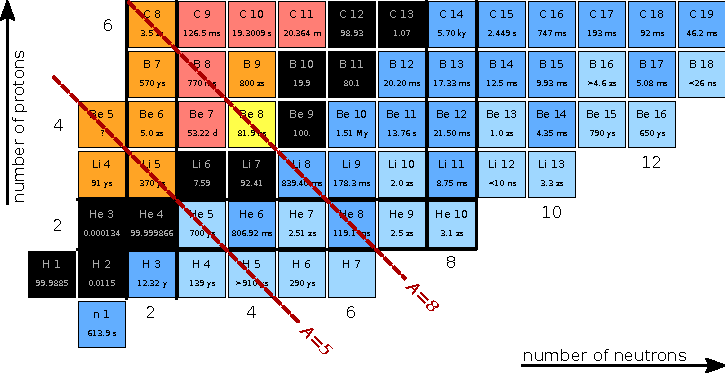
\includegraphics[width=0.85\textwidth]{graphics/bbn/chart_nuclides_bbn}
    \caption{The low-mass section of the chart of the nuclides with red, dashed lines indicating $A=5$ and $A=8$. These are the two mass regions that do not have any stable nuclides, thus effectively halting heavier element production in \ac{bbn}. Chart generated with a \href{https://github.com/kmiernik/Chart-of-nuclides-drawer}{python tool by Krzysztof Miernik}.}
    \label{fig:bbn:chart_nuclides_low_mass_region}
\end{figure}
Figure~\ref{fig:bbn:chart_nuclides_low_mass_region} shows an excerpt of the chart of the nuclides from hydrogen to carbon. Black isotopes are stable. The dashed, red lines indicate mass numbers $A=5$ and $A=8$, at which no stable nuclides exist. Thus, reactions of two \ex{4}He nuclei or a \ex{4}He nucleus and a proton do not form stable nuclides, which prevents \ac{bbn} from forming anything heavier than \ex{7}Li. 

While nucleosynthesis takes place, the universe continues expanding, thus the temperature further decreases. This significantly limits the time in which new nuclides can form. Below a temperature of $T_9\approx 0.1$ \ac{bbn} comes to a halt. This means that around 10-15\,min after the Big Bang, all the hydrogen, helium, and other \ac{bbn} products were formed. 

\begin{figure}[tb]
    \centering
    
\includegraphics[width=0.4\textwidth]{graphics/bbn/reaction_network}
    \caption{\ac{bbn} reaction rate network for dominant reactions, after \citet{nollett2000}.}
    \label{fig:bbn:reaction_network}
\end{figure}
Figure~\ref{fig:bbn:reaction_network} shows the reaction network showing dominant reactions at work in \ac{bbn} \citep[after][]{nollett2000}. As is common, we abbreviate the \ex{4}He nucleus with the symbol $\alpha$. Reactions are written in their abbreviated form, as is common in nuclear physics. For example \ex{1}H(n,$\gamma$)\ex{2}H could also be written as \ex{1}H + n $\longrightarrow$ \ex{2}H + $\gamma$. Notably, there is no main reaction to produce \ex{6}Li. Lithium-7 can be produced in two ways: directly from tritium by capturing a $\alpha$ particle (which is equivalent to \ex{4}He capturing a tritium nucleus) or by production of \ex{7}Be (from \ex{3}He) and subsequent decay to \ex{7}Li.


\subsection{Observational Constraints}

So far, we have roughly derived the production of hydrogen and \ex{4}He expected to form during the Big Bang. We furthermore mentioned how D, \ex{3}He, and \ex{7}Li are produced. Our derivations were mainly based on the temperature and density evolution of the universe during \ac{bbn}, two quantities that are coupled to each other. By observing the abundances of hydrogen, helium, and lithium in the universe and deriving the fractions of the species of interest that formed in the Big Bang, we can constrain the environment in which \ac{bbn} took place. 

\begin{figure}[tb]
    \centering
    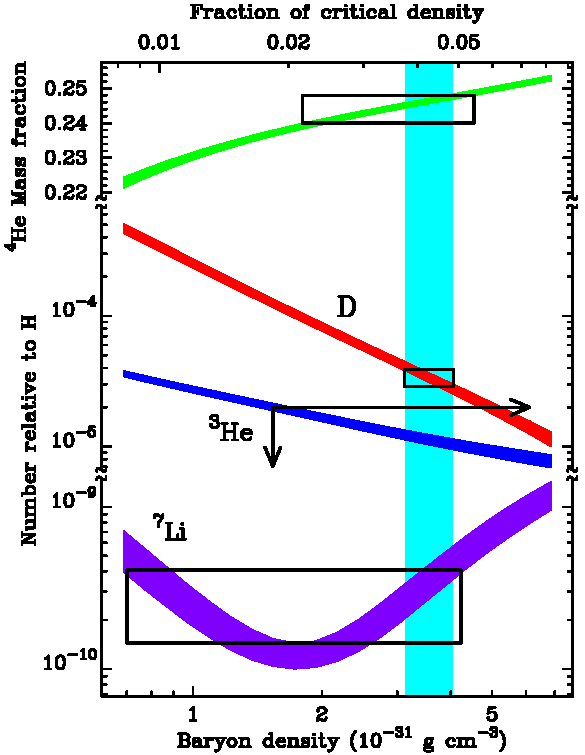
\includegraphics[width=0.5\textwidth]{graphics/bbn/tytler2000_fig2}
    \caption{\ac{bbn} predictions of the D, \ex{3}He, \ex{4}He, and \ex{7}Li abundance as a function of the present-day baryon density \citep{tytler20}. From \href{https://arxiv.org/abs/astro-ph/0001318}{\texttt{arXiv:astro-ph/0001318}}.}
    \label{fig:bbn:nuclides_baryon_density}
\end{figure}
Figure~\ref{fig:bbn:nuclides_baryon_density} shows the calculated abundances of D, \ex{3}He, \ex{4}He, and \ex{7}Li when varying the present-day baryon density. The squares show the observed ratios, where available, and their uncertainties. The larger the baryon density in the universe, the larger is the baryon-to-photon ratio. As discussed before, this ratio and the temperature define when deuterium can form (see Figure~\ref{fig:bbn:planck_radiation_deuterium_fusion}). If the baryon-to-photon ratio goes up, fewer neutrons decay until they are captured and thus more \ex{4}He nuclei are ultimately formed. The conversion of D to \ex{4}He will also be more complete, thus less deuterium remains. The higher starting abundance of D and higher end abundance of \ex{4}He also results in burning out \ex{3}He more effectively, thus lowering its abundance with an increase in the baryon density. The curve in Figure~\ref{fig:bbn:nuclides_baryon_density} for \ex{7}Li shows the competition of two reactions. At low baryon densities, \ex{7}Li is mainly produced via \ex{4}He + T $\longrightarrow$ \ex{7}Li + $\nu$. At increased baryon density, \ex{7}Li however gets again efficiently destroyed by burning further. This destruction is compensated and overtaken at even higher baryon densities since \ex{7}Be is produced more efficiently, which then immediately decays to \ex{7}Li.

While difficult to observe, the abundance of \ac{bbn}-produced hydrogen, helium, and lithium in the universe is a great way to determine crucial parameters of the Big Bang model. Similar insights can however also be gained by analyzing the \ac{cmb}.

\section{Recombination}

In Section~\ref{sec:bbn:standard_model:assumptions} we laid out the assumptions of the standard model of cosmology, one of which is that the overall charge in the universe is zero. During \ac{bbn}, the temperature too high to for electrons and nuclei to combine in order to produce a neutral gas. These components thus rather occur as a plasma. In order to create a neutral gas, the temperature has to sink to below $3000$\,K. At this temperature, the electrons combine with the atomic nuclei. Historically, this phase has been described as recombination, although the ``re'' part is slightly misleading since electrons and nuclei have never been combined previously.

During the plasma phase, i.e., prior to recombination, photons can scatter easily and the universe is thus opaque. After recombination the universe becomes transparent, and we transition into the matter dominated universe (see Figure~\ref{fig:bbn:cosmology_phases}). Since the Big Bang, roughly $4\times10^{5}$\,a have elapsed at this point.

The transition from the radiation dominated to the matter dominated universe can still be seen today as the horizon of the visible universe. It has significantly cooled down and is today seen as the \ac{cmb}. An image of is fluctuations is shown in Figure~\ref{fig:bbn:wmap_cmb}.


\section{Reading}

Since \ac{bbn} took place fairly long ago at this point, it seems adequate to also look at the literature from a historic point of view. For the historical perspective one should read \citet{alpher48} and \citet{peebles66prl}. These are both fairly short manuscripts. The present status of \ac{bbn} was recently given by \citet{cyburt16}. While this work contains fairly detailed methods on uncertainty calculations that are outside the scope of this lecture, please read sections III. Observations and V. The Lithium Problem in detail. You might also want to skim the introduction and the preliminaries.

For these readings it is important that you do not get hung up on details you do not understand, but rather try to follow the big picture. The following questions that can be discussed in class might help to focus on the big picture.

\begin{itemize}
    \item What elements and isotopes are all formed in the Big Bang according to the work by \citet{alpher48}? What are the issues you see with this model, especially regarding it from the current state of knowledge?
    \item What nuclides were produced in the Big Bang according to \citet{peebles66prl} and how does this differ from the work by \citet{alpher48}?
    \item Note the neutron half-life that is used in \citet{peebles66prl}. What is the issue here? This is also in detail discussed in the introduction by \citet{cyburt16}.
    \item What importance does the nuclear reaction rate network have in \citet{cyburt16}? What reaction rates are to this day fairly uncertain?
    \item Discuss how the primordial abundance of H, D, \ex{3}He, \ex{4}He, and \ex{7}Li can be derived from current observations. What are the problems?
    \item What is meant in \citet{cyburt16} by ``regression to zero metallicity''?
\end{itemize}


% Bibliography

\phantomsection
\addcontentsline{toc}{chapter}{Bibliography} \label{sec:bibliography}
\bibliographystyle{aasjournal}
\bibliography{origin_elements}

\end{document}